\section{Set-Up}
For the study of the QHE a two-dimensional or quasi two-dimensional system is needed.
In this experiment a quantum well is created by confining electrons in a thin layer of HgTe between
two layers of HgCdTe. At low temperatures, all electrons are located in the lowest energy level of the 
two dimensional quantum well. This creates a confinement in the layer stacking direction.
Inside the quantum film of HgTe, the electrons form a two-dimensional electron gas (2DEG) with high mobility.
All measurements are done in a variable temperature insert (VTI), which allowes to cool the sample down to a
range between roughly $4.2\,\text{K}$ and $1.5\,\text{K}$. The sample is designed in a common Hall bar geometry,
with in total $8$ contacts on the edges with a additional pair for the Gate voltage (see fig.\,\ref{fig:HallBar})
\begin{figure}[h]
    \centering
    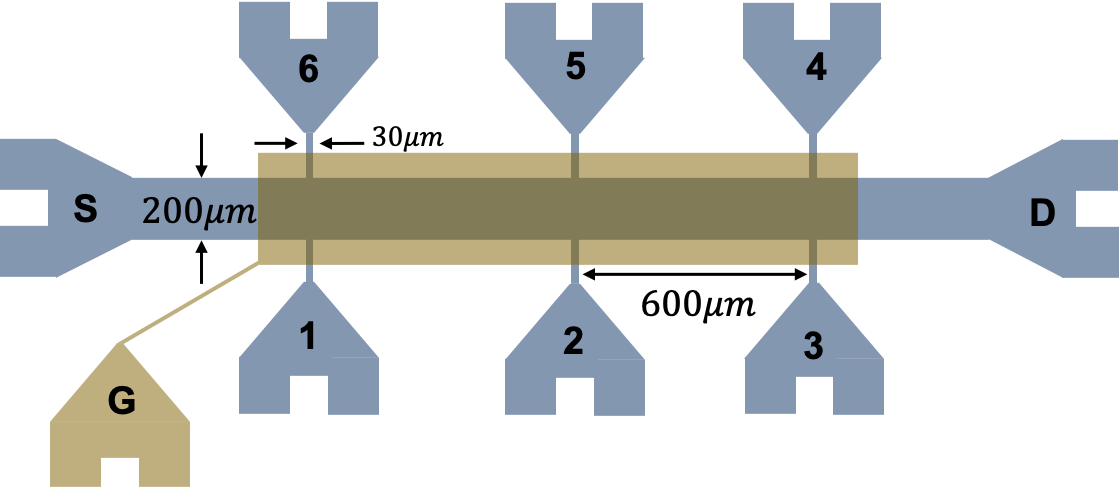
\includegraphics[width=0.45\textwidth]{../Images/HallBar.png}
    \caption{Schematic of the Hall bar geometry. The contacts are labeled with "S" for source, "D" for drain,
    "G" for gate. Contacts $1,3,4$ and $6$ are used for the measurements of $\rho_\text{xx}$ and $\rho_\text{xy}$, 
    whereas contacts $2$ and $5$ are solely used for insurance of homegenity.}
    \label{fig:HallBar}
\end{figure}